% ------------------------------------------------------------
% Page 74
% ------------------------------------------------------------

Mon arrière grand père, \textbf{Louis Couderc}, tisserand à Meyrueis au Ferradou
connaissant bien Saumade et le Moulin d’Ayres, pour qui il avait travaillé, se
porta acquéreur pour la somme de 9.000 Fr. L’acte de vente fut signé le 26 Mai
1890. (4.000 Fr. furent payés comptant et 5.000 exigibles à la fin Septembre
1893, plus, bien entendu, l’intérêt fixé à 4\% l’an).

\vspace{0.35cm}

C’était une grosse somme et Louis Couderc eut du mal à réunir ces 5.000 Fr.
gagnés par un travail acharné et une vie très austère. (sa fille, Emma Couderc-
Loupiac disait « n’avoir pas toujours mangé à sa faim ») ; au point qu’il
envisagea de revendre le Moulin. Finalement il resta dans la famille, et la
filature fit d’assez bonnes affaires ; la famille connut une certaine aisance
d’autant plus que \textbf{Paul Loupiac}, mari d’Emma, mon grand père, très compétent
avait pris la direction.

\vspace{0.35cm}

Mais la guerre déclarée, en Août 1914 affecta fortement Louis Couderc (son
gendre Paul fut mobilisé dans la territoriale en Ariège et un de ses neveux Albert,
fut tué à la bataille de Soissons en 1915). Louis Couderc avait repris les rênes
mais il mourut en 1917 : ce fut le début du déclin de la filature et de la plupart de
ces petites industries semblables dans les Cévennes.

\vspace{0.35cm}

Elle redémarra cependant en 1918 avec le retour de Paul Loupiac, démobilisé,
mais une première congestion cérébrale en 1926 suivie de plusieurs rechutes
amena l’arrêt définitif de la filature.

\vspace{0.35cm}

Les machines étaient devenues obsolètes : il eût fallu en racheter de nouvelles,
investir et Frank Loupiac le fils qui aurait désiré rester au pays était trop jeune
et sans moyens financiers Peut être se rendit-il compte que ces petites entreprises,
cardages, moulinages, filatures, chapelleries étaient condamnées par « le progrès
industriel ».

\vspace{0.6cm}

\begin{center}
    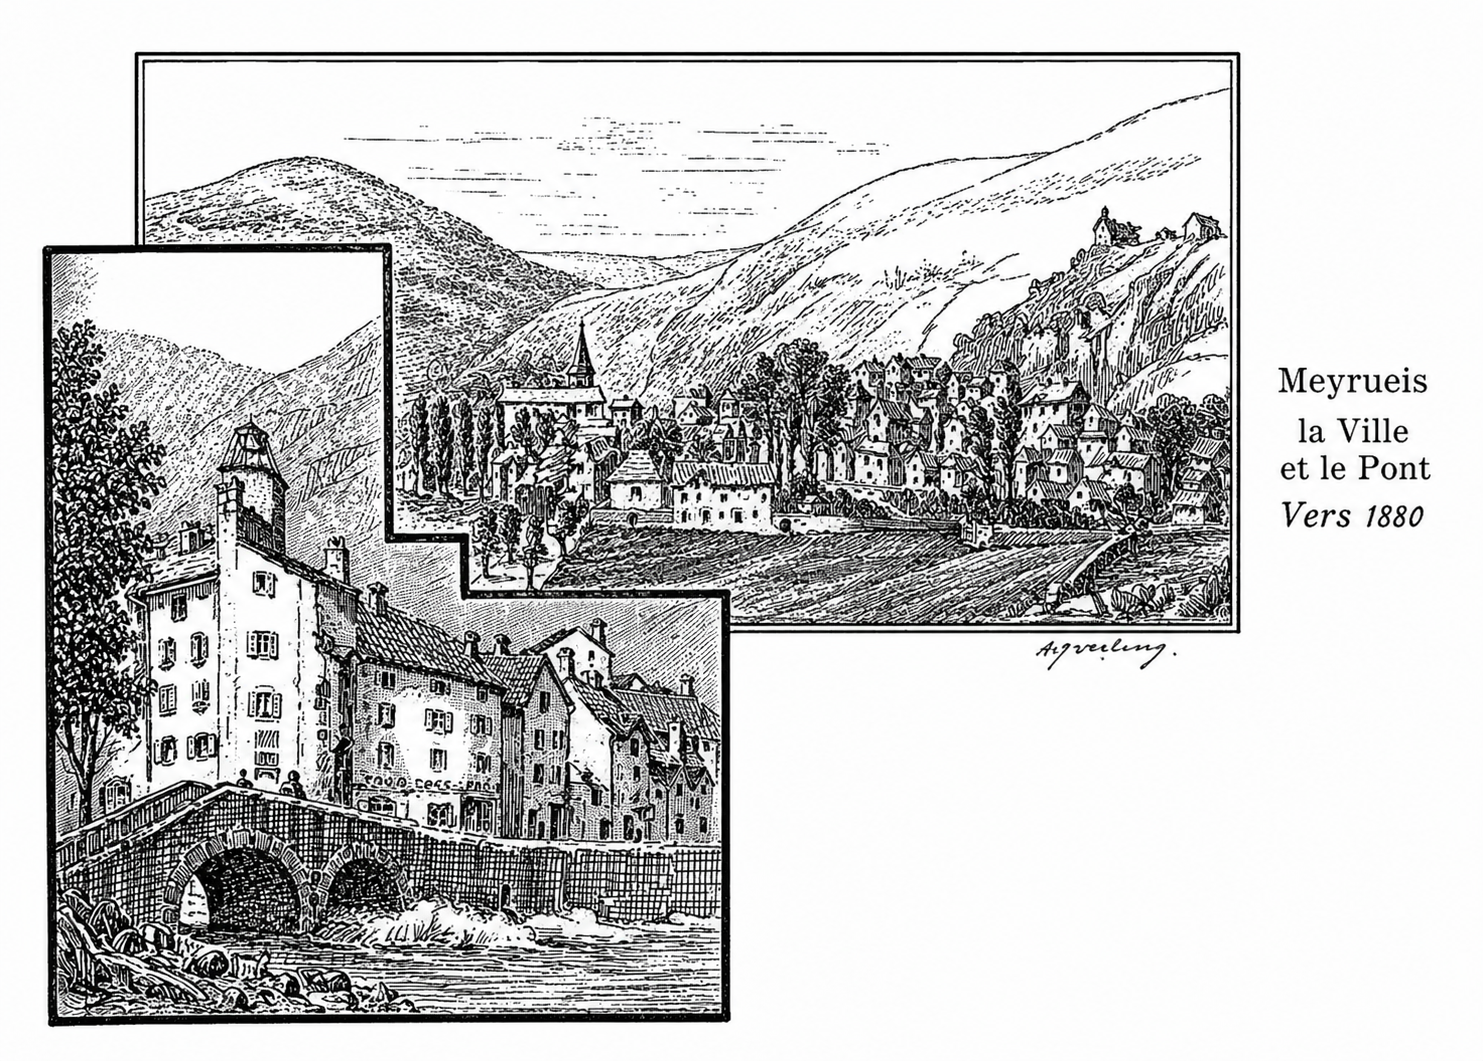
\includegraphics[width=0.9\textwidth]{imgs/078}
\end{center}
